\documentclass[twocolumn, 10pt]{article}
\setlength\textwidth{6.875in}
\setlength\textheight{8.875in}
% set both margins to 2.5 pc
\setlength{\oddsidemargin}{-0.1875in}% 1 - (8.5 - 6.875)/2
\setlength{\evensidemargin}{-0.1875in}
\setlength{\marginparwidth}{0pc}
\setlength{\marginparsep}{0pc}%
\setlength{\topmargin}{0in} \setlength{\headheight}{0pt}
\setlength{\headsep}{0pt}
\setlength{\footskip}{37pt}%
%\setlength{\columnsep}{0.3125in}
%\setlength{\columnwidth}{3.28125in}% (6.875 - 0.3125)/2 = 3.28125in
\setlength{\parindent}{1pc}
\newcommand{\myMargin}{1.00in}
\usepackage[top=\myMargin, left=\myMargin, right=\myMargin, bottom=\myMargin, nohead]{geometry}
\usepackage{epsfig,graphicx}
\usepackage{palatino}
\usepackage{fancybox}
\usepackage{hyperref}
\usepackage[procnames]{listings}

% "define" Scala
\usepackage[T1]{fontenc}  
\usepackage[scaled=0.82]{beramono}  
\usepackage{microtype} 

\sbox0{\small\ttfamily A}
\edef\mybasewidth{\the\wd0 }

\lstdefinelanguage{scala}{
  morekeywords={abstract,case,catch,class,def,%
    do,else,extends,false,final,finally,%
    for,if,implicit,import,match,mixin,%
    new,null,object,override,package,%
    private,protected,requires,return,sealed,%
    super,this,throw,trait,true,try,%
    type,val,var,while,with,yield},
  sensitive=true,
  morecomment=[l]{//},
  morecomment=[n]{/*}{*/},
  morestring=[b]",
  morestring=[b]',
  morestring=[b]"""
}

\usepackage{color}
\definecolor{dkgreen}{rgb}{0,0.6,0}
\definecolor{gray}{rgb}{0.5,0.5,0.5}
\definecolor{mauve}{rgb}{0.58,0,0.82}

% Default settings for code listings
\lstset{language=scala,
  showstringspaces=false,
  columns=fixed, % basewidth=\mybasewidth,
  basicstyle={\small\ttfamily},
  numbers=none,
  numberstyle=\footnotesize\color{gray},
  % identifierstyle=\color{red},
  keywordstyle=\color{blue},
  commentstyle=\color{dkgreen},
  stringstyle=\color{mauve},
  breakatwhitespace=true,
  procnamekeys={def, val, var, class, trait, object, extends},
  procnamestyle=\ttfamily\color{red},
}

\lstnewenvironment{scala}
{\lstset{language=scala}}
{}
\lstnewenvironment{cpp}
{\lstset{language=C++}}
{}
\lstnewenvironment{bash}
{\lstset{language=bash}}
{}
\lstnewenvironment{verilog}
{\lstset{language=verilog}}
{}

\newcommand{\isc}{
\lstinline
}

\lstdefinestyle{scala}{language=scala,
  showstringspaces=false,
  columns=fixed, % basewidth=\mybasewidth,
  basicstyle={\small\ttfamily},
  numbers=none,
  numberstyle=\footnotesize\color{gray},
  % identifierstyle=\color{red},
  keywordstyle=\color{blue},
  commentstyle=\color{dkgreen},
  stringstyle=\color{mauve},
  breakatwhitespace=true,
  procnamekeys={def, val, var, class, trait, object, extends},
  procnamestyle=\ttfamily\color{red},
}


\lstset{basicstyle={\footnotesize\ttfamily}}

\newenvironment{commentary}
{ \vspace{-0.1in}
  \begin{quotation}
  \noindent
  \small \em
  \rule{\linewidth}{1pt}\\
}
{
  \end{quotation}
}

\title{Getting Started - Tutorial 03: Instantiating Modules}
\author{Jonathan Bachrach, Vincent Lee \\
EECS Department, UC Berkeley\\
{\tt  \{jrb\}@eecs.berkeley.edu}
}
\date{\today}

\newenvironment{example}{\VerbatimEnvironment\begin{footnotesize}\begin{Verbatim}}{\end{Verbatim}\end{footnotesize}}
\newcommand{\kode}[1]{\begin{footnotesize}{\tt #1}\end{footnotesize}}

\def\code#1{{\tt #1}}

\def\note#1{\noindent{\bf [Note: #1]}}
%\def\note#1{}

\begin{document}
\maketitle{}

\section{Module Instantiation}

Like other hardware description languages, Chisel allows fairly straightforward module instantiation to enable modularity and hierarchy. In Chisel, instantiating a Module class is the equivalent to instantiating a module in Verilog. To do this, we simply use a call to \verb+Module+ with module created with the Scala \verb+new+ keyword in order to indicate that we are instantiation a new module. We want to make sure we assign this to a value so that we can reference its input and outputs which we also need to connect.

For example, suppose we would like to construct a 4-bit adder using multiple copies of the  \verb+FullAdder+ module. as shown in the Figure 1. The Chisel source code is shown below.

\begin{figure}[ht!]
\centering
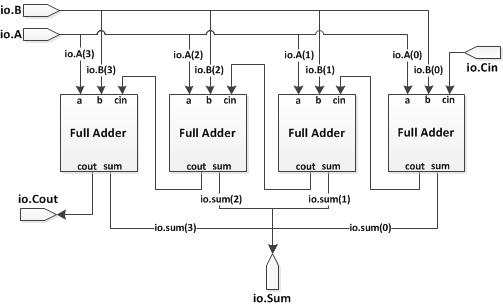
\includegraphics[width=80mm]{figs/4_Bit_Adder.jpg}
\caption{Block Diagram of 4-Bit Adder}
\label{overflow}
\end{figure}

\begin{scala}
// A 4-bit adder with carry in and carry out
class Adder4 extends Module {
  val io = new Bundle {
    val A    = UInt(INPUT, 4)
    val B    = UInt(INPUT, 4)
    val Cin  = UInt(INPUT, 1)
    val Sum  = UInt(OUTPUT, 4)
    val Cout = UInt(OUTPUT, 1)
  }
  // Adder for bit 0
  val Adder0 = Module(new FullAdder())
  Adder0.io.a   := io.A(0)
  Adder0.io.b   := io.B(0)
  Adder0.io.cin := io.Cin
  val s0 = Adder0.io.sum
  // Adder for bit 1
  val Adder1 = Module(new FullAdder())
  Adder1.io.a   := io.A(1)
  Adder1.io.b   := io.B(1)
  Adder1.io.cin := Adder0.io.cout
  val s1 = Cat(Adder1.io.sum, s0)
  // Adder for bit 2
  val Adder2 = Module(new FullAdder())
  Adder2.io.a   := io.A(2)
  Adder2.io.b   := io.B(2)
  Adder2.io.cin := Adder1.io.cout
  val s2 = Cat(Adder2.io.sum, s1)
  // Adder for bit 3
  val Adder3 = Module(new FullAdder())
  Adder3.io.a   := io.A(3)
  Adder3.io.b   := io.B(3)
  Adder3.io.cin := Adder2.io.cout
  io.Sum  := Cat(Adder3.io.sum, s2).toUInt()
  io.Cout := Adder3.io.cout
}
\end{scala}

In this example, notice how when referencing each module I/O we must first reference the \verb+io+ that contains the ports for the I/Os. Again, note how all assignments to the module I/Os use a reassignment operator \verb+:=+. When instantiating modules, it is important to make sure that you connect all the input and output ports. If a port is not connected, the Chisel compiler may optimize away portions of your design that it find unecessary due to the unconnected ports and throw errors or warnings.

\section{The Vec Class}

The \verb+Vec+ class allows you to create an indexable vector in Chisel which can be filled with any expression that returns a chisel data type. The general syntax for a \verb+Vec+ declaration is given by:
\begin{scala}
val myVec = 
  Vec.fill( <number of elements> ) { <data type> }
\end{scala}
Where \verb+<number of elements>+ corresponds to how long the vector is and \verb+<data type>+ corresponds to what type of class the vector contains.

For instance, if we wanted to instantiate a 10 entry vector of 5 bit UInt values, we would use:

\begin{scala}
val ufix5_vec10 := Vec.fill(10) { UInt(width = 5) }
\end{scala}

If we want to define a vector of registers...

\begin{scala}
val reg_vec32 := Vec.fill(32){ Reg() }
\end{scala}

In order to assign to a particular value of the \verb+Vec+, we simply assign the target value to the vector at a specified index. For instance, if we wanted to assign a UInt value of zero to the first register in the above example, the assignment would look like:

\begin{scala}
reg_vec32(1) := UInt(0)
\end{scala}

To access a particular element in the vector at some index, we specify the index of the vector. For example, to extract the 5th element of the register vector in the above example and assign it to some value \verb+reg5+, the assignment would look like:

\begin{scala}
val reg5 = reg_vec(5)
\end{scala}

The syntax for the \verb+Vec+ class is slightly different when instantiating a vector of modules. When instantiating a vector of modules the data type that is specified in the {} braces is slightly different than the usualy primitive types. To specify a vector of modules, we use the \verb+io+ bundle when specifying the type of the vector. For example, in order to specify a \verb+Vec+ with 16 modules , say \verb+FullAdder+s in this case, we would use the following declaration:

\begin{scala}
val FullAdders = 
  Vec.fill(16){ Module(new FullAdder()).io }
\end{scala}

Notice we use the keyword \verb+new+ in the vector definition before the module name \verb+FullAdder+. For how to actually access the \verb+io+ on the vector modules, refer to the next section.

\section{Parametrization}

In the previous Adder example, we explicitly instantiated four different copies of a \verb+FullAdder+ and wired up the ports. But suppose we want to generalize this structure to an n-bit adder. Like Verilog, Chisel allows you to pass parameters to specify certain aspects of your design. In order to do this, we add a parameter in the Module declaration to our Chisel definition.
For a carry ripple adder, we would like to parametrize the width to some integer value \verb+n+ as shown in the following example:

\begin{scala}

// A n-bit adder with carry in and carry out
class Adder(n: Int) extends Module {
  val io = new Bundle {
    val A    = UInt(INPUT, n)
    val B    = UInt(INPUT, n)
    val Cin  = UInt(INPUT, 1)
    val Sum  = UInt(OUTPUT, n)
    val Cout = UInt(OUTPUT, 1)
  }
  // create a vector of FullAdders
  val FAs = Vec.fill(n){ Module(new FullAdder()).io }

  // define carry and sum wires
  val carry = Vec.fill(n+1){ UInt(width = 1) }
  val sum   = Vec.fill(n){ Bool() } 

  // first carry is the top level carry in
  carry(0) := io.Cin

  // wire up the ports of the full adders
  for(i <- 0 until n) {
     FAs(i).a   := io.A(i)
     FAs(i).b   := io.B(i)
     FAs(i).cin := carry(i)
     carry(i+1) := FAs(i).cout
     sum(i)     := FAs(i).sum.toBool()
  }
  io.Sum  := sum.toBits().toUInt()
  io.Cout := carry(n)
}

\end{scala}

Note that in this example, we keep track of the sum output in a \verb+Vec+ of \verb+Bool+s. This is because Chisel does not support bit assignment directly. Thus in order to get the n-bit wide \verb+sum+ in the above example, we use an n-bit wide \verb+Vec+ of \verb+Bool+s and then cast it to a UInt(). Note that it must first be casted to the \verb+Bits()+ type before casting it to \verb+UInt()+.

You will notice that modules are instantiated in a Vec class which allows us to iterate through each module when assigning the ports connections to each \verb+FullAdder+. This is similar to the generate statement in Verilog. However, you will see in more advanced tutorials that Chisel can offer more powerful variations.

Instantiating a parametrized module is very similar to instantiating an unparametrized module except that we must provide arguments for the parameter values. For instance, if we wanted to instantiate a 4-bit version of the \verb+Adder+ module we defined above, it would look like:

\begin{scala}
val adder4 = Module(new Adder(4))
\end{scala}

We can also instantiate the \verb+Adder+ by explicitly specifying the value of it parameter \verb+n+ like the this:

\begin{scala}
val adder4 = Module(new Adder(n = 4))
\end{scala}

Explicitly specifying the parameter is useful when you have a module with multiple parameters. Suppose you have a parametrized FIFO module with the following module definition:

\begin{scala}
class FIFO(width: Int, depth: Int) extends Module {...}
\end{scala}

You can explicitly specify the parameter values in any order:

\begin{scala}
val fifo1 = Module(new FIFO(16, 32))
val fifo2 = Module(new FIFO(width = 16, depth = 32))
val fifo3 = Module(new FIFO(depth = 32, width = 16))
\end{scala}

All of the above definitions pass the same parameters to the FIFO module. Notice that when you explicitly assign the parameter values, they can occur in any order you want such as the definition for fifo3.

\section{Advanced Parametrization}

Although parameters can be passed explicitly through a Module's constructor, this technique does not scale when parameterizing large designs with many parameterized components. For a more detailed explanation of why a better parameterization method is needed, please see XXXX. In addition, XXXX explains heuristics for how to organize and parameterize large designs, which we highly recommend reading prior to using this functionality on complicated designs.

Every Module has its own \verb+params+ object, which acts as a dictionary. Querying this object is shown below.

\begin{scala}
val width = params[Int]('width')
\end{scala}

If \verb+params+ is queried and no parameter matches the query, Chisel throws a \verb+ParameterUndefinedException+. Notice the query return type must be provided.

When a parent Module creates a child Module, the parent's \verb+params+ object is automatically cloned and passed to the child. In the following example, suppose the parent's params object returns \verb+10+ when queried for width. Because the \verb+Parent+ \verb+params+ object is automatically cloned for \verb+Child+, the \verb+Child+ query also returns \verb+10+.

\begin{scala}
class Parent extends Module {
  val io = new Bundle { ... }
  val width = params[Int]('width') // returns 10
  // create child Module implicitly passing params
  val child = Module(new Child) 
}
class Child extends Module {
  val io = new Bundle { ... }
  val width = params[Int]('width') // returns 10
}
\end{scala}

Suppose a parent Module wants to override or add parameters to its child's \verb+params+ object. This case requires adding a partial function (a Scala way of defining key-value mappings) to the \verb+Child+ Module constructor:

\begin{scala}
class Parent extends Module {
  val io = new Bundle { ... }
  val width = params[Int]('width') // returns 10
  val n = params[Int]('n') // returns 20
  val child = Module(new Child,{'n' => 40})
}
class Child extends Module {
  val io = new Bundle { ... }
  val width = params[Int]('width') // returns 10
  val n = params[Int]('n') // returns 40
}
\end{scala}

A more complicated design may have the following structure:

\begin{scala}
class Top extends Module {
  val io = new Bundle { ... }
  val p = Module(new Parent,{
    'width' => 10
    'name' => 'Parent'
  })
}
class Parent extends Module {
  val io = new Bundle { ... }
  val width = params[Int]('width')  // returns 10
  val name = params[String]('name') // returns 'Parent'
  val child1 = Module(new Child,{'name' => 'Child 1'})
  val child2 = Module(new Child,{'name' => 'Child 2'})
}
class Child extends Module {
  val io = new Bundle { ... }
  val width = params[Int]('width')  // returns 10
  val name = params[String]('name') // returns 'Child 1'
                                    //   or 'Child 2'
}
\end{scala}

For more advanced uses, tips, and tricks, please see XXXX.

\section{Built In Primitives}

Like other HDL, Chisel provides some very basic primitives. These are constructs that are built in to the Chisel compiler and come for free. The Reg, UInt, and Bundle classes are such primitives that has already been covered. Unlike Module instantiations, primitive do not require explicit connections of their io ports to use. Other useful primitive types include the Mem and Vec classes which will be discussed in a more advanced tutorial. In this tutorial we explore the use of the \verb+Mux+ primitive

\subsection{The Mux Class}

The \verb+Mux+ primitive is a two input multiplexer. In order to use the \verb+Mux+ we first need to define the expected syntax of the \verb+Mux+ class. As with any two input multiplexer, it takes three inputs and one output. Two of the inputs correspond to the data values \verb+A+ and \verb+B+ that we would like to select which can be any width and data type as long as they are the same. The third input \verb+select+ which is a Bool type determines which one to output.
A \verb+select+ value of \verb+true+ will output the first value \verb+A+, while a \verb+select+ value of \verb+false+ will pass \verb+B+.

\begin{scala}
val out = Mux(select, A, B)
\end{scala}

Thus if \verb+A=10+, \verb+B=14+, and \verb+select+ was \verb+true+, the value of \verb+out+ would be assigned 10. Notice how using the \verb+Mux+ primitive type abstracts away the logic structures required if we had wanted to implement the multiplexer explicitly.

% Martin: I would drop the following as it is just confusing in a tutorial
% state simple that there is a Mux primitive and that is fine.

%The instantiation would look something like this:
%
%\begin{scala}
%// where n is the width of A and m is the width of B
%val mux = Module(new Mux(n, m))
%mux.io.select := select
%mux.io.A      := A
%mux.io.B      := B
%val out = mux.io.out
%\end{scala}
%
%We see that clearly it is much cleaner to use the primitive \verb+Mux+ type instead of trying to write and implement our own general multiplexer since the \verb+Mux+ type does all the wiring for you.


%\section{Exercises}
%
%\subsection{n-bit Subtractor}
%
%Earlier in this tutorial we demonstarted how to parametrize and instantiate an n-bit ripple adder. <Finish this>
%


\end{document}
